\section{783 --- Minimum Distance Between BST Nodes}
Given a Binary Search Tree (BST) with the root node \fcj{root}, return the minimum difference between the values of any two different nodes in the tree.

\paragraph{Example:}
\begin{flushleft}


\textbf{Input}: \fcj{root = [4,2,6,1,3,null,null]}

\textbf{Output}: 1

\textbf{Explanation}:

Note that root is a TreeNode object, not an array.

The given tree \fcj{[4,2,6,1,3,null,null]} is represented by the following diagram:

\begin{figure}[H]
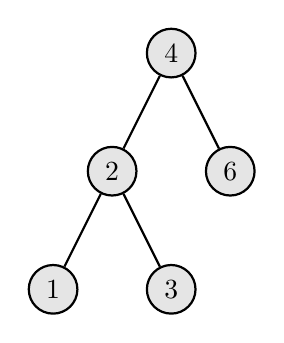
\begin{tikzpicture}
[every node/.style={draw, circle, fill=gray!20!, minimum size=5mm},
%level 1/.style={sibling distance=25mm},
%level 2/.style={sibling distance=15mm},
thick]
\node{4}
child{node{2} child{node{1}} child{node{3}}}
child{node{6}};
\end{tikzpicture}
\end{figure}


while the minimum difference in this tree is 1, it occurs between node 1 and node 2, also between node 3 and node 2.
\end{flushleft}
\paragraph{Note:}


\begin{enumerate}
\item The size of the BST will be between 2 and 100.
\item The BST is always valid, each node's value is an integer, and each node's value is different.
\end{enumerate}

\subsection{Inorder}
Inorder traversing of BST will give ascending order of values. The minimum difference only happens between two consecutive values.

\setcounter{lstlisting}{0}
\begin{lstlisting}[style=customc, caption={Inorder Traverse}]
int minDiffInBST( TreeNode* root )
{
    auto ans( INT_MAX );
    int pre = -1;
    //this flag indicate if pre is set
    bool flag = false;
    inorder( root, pre, flag, ans );
    return ans;
}
void inorder( TreeNode* node, int& pre, bool& flag, int& ans )
{
    if( !node )
    {
        return;
    }
    inorder( node->left, pre, flag, ans );
    if( !flag )
    {
        pre = node->val;
        flag = true;
    }
    else
    {
        ans = ( min )( node->val - pre, ans );
        pre = node->val;
    }
    inorder( node->right, pre, flag, ans );
}
\end{lstlisting}